\chapter{Úvod}

\section{Motivácia}
Väčšina modelov v strojovom učení predikuje alebo klasifikuje iba na základe aktuálneho vstupu pričom neberie do úvahy predchádzajúce vstupy. Existujú však úlohy pri ktorých potrebujeme brať do úvahy aj predchádzajúce stavy z minulých vstupov, čo nazývame kontext. 
Predstavme si napríklad, že chceme sieť naučiť predikovať ďalšie písmeno v slove. Ako príklad si vezmime slovo "java". Trénovanie nerekurentnej siete by prebiehalo nasledujúcim spôsobom: sieti dám písmeno "j" a poviem, že očakávam "a" a takto pokračujem ďalej. Problém nastane pri písmene "v", kde opäť očakávam "a", ale sieť je už naučená, že pímeno "a" nasleduje po "j". Je zrejmé, že na vyriešenie tohto problému potrebujem brať do úvahy aj nejaký historický kontext, teda stavy siete z predchádzajúcich krokov.
Takýto druh neurónovej siete sa nazýva rekurentná neurónová sieť.

V našej diplomovej práci budeme skúmať hĺbku pamäte rôznych typov neurónových sietí. 

\section{Prehľad literatúry a úvod do problematiky}
\subsection{Samoorganizujúce sa mapy}
Je to typ neurónovej siete, v ktorej sú jednotlivé neuróny usporiadané v štvorcovej mriežke. Samoorganizujúce sa mapy (ďalej iba SOM) sú trénované bez učiteľa, čiže váhy jednotlivých neurónov sú upravované iba na základe dát z trénovacej množiny. Čo je zaujímavé na spôsobe trénovania SOM je, že je veľmi podobný učeniu neurónov v mozgovej kôre živočíchov.

Špeciálnou vlastnosťou SOM je, že po natrénovaní zobrazí trénovaciu množinu so zachovanou topológiou. To znamená, že blízke (podobné) vstupy aktivujú blízke neuróny v sieti. Vzdialenosť dvoch neurónov je ich euklidovská vzdialenosť v mriežke. Takéto topologické zobrazenie dát sa vyskytuje aj v biologických neurónových sieťach.

\subsection{Trénovanie}
Trénovanie SOM je založené na tzv. Hebbovom pravidle učenia, ktoré znie nasledovne:
Keď má axón bunky A excitačný účinok na bunku B, a opakovane sa zúčastňuje na jej aktivácii, v jednej
alebo v oboch bunkách prebehne určitý rastový proces alebo metabolická zmena, takže účinnosť bunky A ako jednej z buniek, ktoré aktivujú B, vzrastie.
Proces trénovania SOM je zložený z dvoch častí:
\begin{itemize}
\item hľadanie víťaza
\item adaptácia váh neurónov
\end{itemize}
Na začiatku su váhy medzi vstupom a neurónmi v mriežke inicializujú na náhodné hodnoty z určitého intervalu.
V každom kroku trénovania nájdeme najskôr víťazný neurón pre daný vstup. Postupne počítam euklidovské vzdialenosti vstupu od váhového vektora jednotlivých neurónov. Víťazom je neurón, ktorý je najbližšie k vstupu (má najkratšiu vzdialenosť).

\begin{equation}
i^* = argmin_i||x-w_i|| 
\end{equation}

Druhým krokom je adaptácia váh víťazného neurónu a jeho okolia. Pravidlo pre zmenu váh neurónov:

\begin{equation}
w_i(t+1) = w_i(t) + \alpha(t)h(i^*, i)([x(t) - w_i(t)]
\end{equation}

Váhové vektory víťazného neurónu a jeho topologických susedov sa posúvajú smerom k aktuálnemu vstupu.
$\alpha(t)$ predstavuje rýchlosť učenia, ktorá sa môže klesať v čase alebo môže zostať konštantná. Na funkcii, ktorá je použitá pre $\alpha$ v praxi veľmi nezaléží, mala by to byť nejaká monotónne klesajúca funkcia (napríklad exponenciálna funkcia). 
$h(i^*, i)$ je funkcia okolia (tzv. excitačná funkcia), ktorá definuje koľko neurónov v okolí víťaza bude trénovaných a do akej miery. Inými slovami, excitačná funkcia definuje rozsah kooperácie medzi neurónmi. Používajú sa najčastejšie 2 typy okolia:
\begin{itemize}
\item pravouhlé(štvorcové) okolie

\[
N(i^{*},i) =
     \begin{cases}
       \text{1} &\quad\text{ak } d_{M}(i^*, i) \leq \lambda(t) \\
       \text{0} &\quad\text{inak}\\
     \end{cases}
\]
\\
$d_{M}(i^{*}, i)$ je Manhattanovská vzdialenosť (L1 norma) medzi neurónmi v mriežke mapy. Kohonen zistil, že najlepšie výsledky sú dosiahnuté, keď
sa veľkosť okolia s časom postupne zmenšuje.
\item gaussovské okolie
	\begin{equation}
		N(i^{*}, i) = \exp^{- \frac{d^{2}_{E}(i^{*}, i)}{\lambda^{2}(t)}}
	\end{equation}
$d_{E}(i^{*}, i)$ je euklidovská vzdialenosť (L2 norma) neurónov v mriežke. Funkcia $\lambda^2(t)$ sa s časom postupne zmenšuje až k nule. Táto
	funkcia slúži na zmenšovanie okolia víťazného neurónu počas trénovania, čím sa zabezpečí ukončenie učenia.
\end{itemize}

Pri učení rozlišujeme všeobecne dve fázy:
\begin{itemize}
	\item usporiadavanie - s časom klesá veľkosť okolia víťazných neurónov 
	\item dolaďovanie - veľkosť okolia sa zafixuje na nejakej malej hodnote až pokým učenie neskončí.
\end{itemize}

Kohonen odhadol na základe pokusov, že počet iterácií trénovania, by mal byť rádovo 500-násobok počtu neurónov v sieti.
Rovnako sa pozorovaním zistilo, že na fázu doladenia je lepšie ponechať viac času ako na fázu usporiadavania.

Počas trénovania SOM môžu nastať špeciálne situácie:

\begin{itemize}
	\item Sieť je neúplne rozvinutá - príliš rýchle zmenšovanie rýchlosti učenia $\alpha$
	\begin{figure}[H]
		\caption{Neúplne rozvinutá sieť}
		\centering
		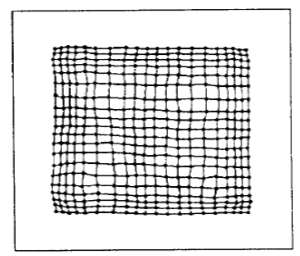
\includegraphics[width=8cm]{assets/too_fast}
	\end{figure}
	
	\item Motýlí efekt - príliš rýchle zmenšovanie okolia $\lambda$
	\begin{figure}[H]
		\caption{Motýlí efekt}
		\centering
		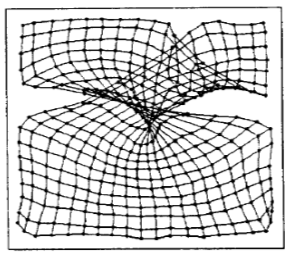
\includegraphics[width=8cm]{assets/butterfly_effect}
	\end{figure}
	
	\item Pinch efekt - príliš pomalé zmenšovanie okolia $\lambda$
	\begin{figure}[H]
		\caption{Pinch effect}
		\centering
		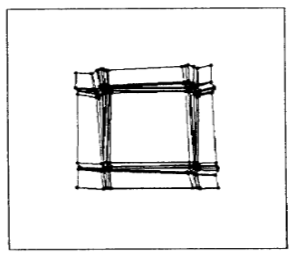
\includegraphics[width=8cm]{assets/pinch_effect}
	\end{figure}
\end{itemize}



\subsection{Využitie SOM}
\begin{itemize}
\item SOM môžeme využiť na mapovanie viacrozmerných dát do 2D - môžeme ju použiť na redukciu dimenzie dát.
\item SOM je aj vektorovým kvantifikátorom. Pri vektorovej kvantizácii nahrádzame množinu vektorov vstupných dát menšou množinou vektorov (nazývaných aj prototypy). V SOM sú prototypmi
		váhové vektory. Toto je možné využiť napríklad na kompresiu dát. Vďaka vektorovej kvantizácii stačí uchovať iba množinu prototypov a informáciu o tom, ktorý vstupný vektor patrí 
		ku ktorému prototypu(centru). Ku každému centru sa potom priradí množina vstupných vektorov, ktoré ku nemu majú bližšie ako ku akémukoľvek inému centru. (používa sa euklidovská vzdialenosť).
		Vektorou kvantizáciou teda rozdelíme vstupný priestor an disjunktné oblasti, ktoré tvoria tzv. Voronoiho mozaiku
\end{itemize}



\subsection{RecSOM}
Rekurentná som je modifikáciou


\subsection{mSOM}
mSOM



\section{Štruktúra ďalšej práce}
\section{Typy neurónových sietí}
\begin{itemize}
	\item elmanova sieť
	\item recSOM
	\item mergeSOM
\end{itemize}
\section{Elmanova sieť a backpropagácia v čase}
Jednoduchú Elmanovu sieť nie je vhodné trénovať pomocou jednoduchécho algoritmu spätného šírenia chyby, pretože neberie do úvahy spätné šírenie chybového signálu cez rekurentné prepojenia do predchádzajúcich časových krokov.
Môže byť však použitý na porovnanie s inými algoritmami pri vyhodnocovaní výsledkov.

Pri algoritme spätného šírenia chyby v čase musíme akokeby rozvinúť rekurentnú sieť do mnohovrstvovej doprednej siete (každý časový krok) a na takto rozvinutú sieť aplikovať algoritmus spätného šírenia chyby.
\section{Meranie hĺbky pamäte samorganizujúcich sa máp}
Ako trénovaciu množinu budem používať sekvenciu písmen abecedy (26 písmen).
Vstupmi (trénovacie príklady) pre sieť budú zakódované jednotlivé písmená z trénovacej sekvencie.
Písmená kódujem do 26 prvkového vektora, ktorého prvky budú nuly a jednotka (pre každé písmeno na inej pozícii).
Každý neurón bude mať množinu v ktorej si bude pamätať pre aký vstup bol víťazom. Nebude si však ukladať iba konkrétne písmeno zo vstupu, ale $k$ posledných písmen z trénovacej množiny (tzv. sliding window). 
Z toho si viem ďalej vytvoriť hitmapu, ktorá mi bude vizualizovať, na aké vstupy neuróny reagovali.
Mierou hĺbky pamäte mapy bude potom vážený priemer dĺžky najdlhších spoločných podpostupností písmen v množinách jednotlivých neurónov. Dĺžku najdlhšej podpostupnosti budem určovať od konca sekvencií v množine. Priemer pamäťových hĺbok jednotlivých neurónov musí byť vážený, aby neuróny s väčším počtom víťazov mali vyššiu váhu ako neuróny s menším počtom víťazov.
Po každej trénovacej epoche (prechode trénovacou množinou) budem vedieť určiť pamäťovú hĺbku mapy.
Vďaka tomu, že neuróny rekurentných sietí majú okrem normálnych váh aj kontextové váhy, ktoré uchovávajú informáciu z predchádzajúceho kroku,  môže sa stať, že rovnaké písmeno zo vstupu bude mať rôzne víťazné neuróny počas trénovania.










